\cref{chapter:nv} concerned a two-qubit approximation of the short-time dynamics of an \gls{nvc}. 
It is valid criticism that the corresponding \gls{model space} searched was reduced substantially through prior knowledge,
    and it therefore remains to test \gls{qmla} in a large model space, on physically meaningful data. 
In this chapter, we extend \gls{qmla} to consider appoximations of \gls{nvc} sytems using more qubits, 
    representing several nuclear sites, which aim to capture the interactions between the 
    target \gls{nvc} and the environment more thoroughly. 
Here we will simulate the target system, allowing us to make definite statements on the performance of \gls{qmla}, 
    unlike the experimental data where we can not be sure of the dynamics' generator.

\par 

\section{Target system}

\begin{figure}
    \begin{center}
        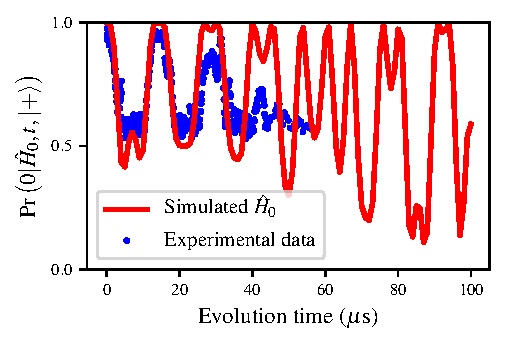
\includegraphics{experimental_study/figures/nv_revival_raw_data.pdf}
    \end{center}
    \caption[Long-time dynamics for nitrogen-vacancy centres]{
        Long-time dynamics for \acrlong{nvc}, red, showing revivals, 
            generated by $\ho$ from \cref{eqn:nv_gen_alg_target}, via Hahn echo measurement with $t^{\prime} = t$.
        For comparison, experimentally generated dynamics are shown in blue. 
    }
    \label{fig:nv_revival_raw}
\end{figure}
A realistic model may be expected from considering the environment as a finite-size bath, 
    consisting of $n_s$ nuclear spins in addition to the \gls+{nvc} spin, 
    i.e. the total number of qubits of such a model is $n_q = 1 + n_s$.   
The effects of nuclear spins are expected to manifest at higher times than those studied in \cref{chapter:nv}, 
    i.e. the decoherence of the \gls{nvc} is only effected by the nuclear spins' independent precession at high times, 
    so we must modify the experimental procedure accordingly.
Such effects can also be highlighted by Hahn echo measurements, 
    as in \cref{fig:hahn_bloch_spheres}, 
    except reversing the evoluting by $t^{\prime} = t$ instead of $t^{\prime} = 2t$
    \cite{breuer2002theory, childress2006coherent}, so our simulations will use this measurement scheme. 
    % TODO reference that explicitly says Hahn t=t' gives long-time dynamics
\par 

Since we are simulating the target system, we may choose the approximation we wish to invoke. 
Starting from the \gls{hamiltonian} expected to describe \glspl{nvc} in \cite{smeltzer201113c}, 
    we again exclude the zero-field and quadrupole splitting (as in \cref{eqn:nv_ham_full}),
    and assume the complete \gls{hamiltonian} to describe the long-time dynamics of an \gls{nvc}, 
\begin{equation}
    \label{eqn:complete_long_dynamics_nv_model}
    \hat{H}_{\textrm{long}} =
    \mu_B g \mathbf{B} \cdot \mathbf{S} 
    + \gamma \cdot \mathbf{B} \cdot \mathbf{I} 
    + \mathbf{A} \cdot \mathbf{S} \cdot \mathbf{I},
\end{equation}
    where\footnotemark 
\begin{easylist}[itemize]
    & $\mu_B = 9.274 \times 10^{-24} \SI{}{\joule\per\tesla}$ is the Bohr magneton;
    & $g \approx 2$ is the electron $g$-factor;
    & $\mathbf{B}$ is the magnetic field with magnitude $B=\SI{11}{\milli\tesla}$;
    & $\mathbf{S}$ is the total electron spin operator;
    & $\mathbf{I}$ is the total nuclear spin operator.
    & $\gamma$ is gyromagnetic ratio, 
        with dominant axial contributions from $^{13}C$ of $\gamma_z = \SI{10.8}{\mega\hertz\per\tesla}$
        and nonaxial contribution from proximal nuclei of $\gamma_x = \gamma_y = \SI{42.6}{\mega\hertz\per\tesla}$ \cite{kubala2016hyperpolarized};
    & $\mathbf{A}$ is the hyperfine tensor, coupling the electron with the nuceli, 
        here we take it to consist of $A = A_x = A_y = A_z = \SI{0.2}{\mega\hertz}$ \cite{felton2009hyperfine}.
\end{easylist}
\footnotetext{Note: the parameter values used here do not necessarily correspond to a physical system as they are 
    taken from a range of sources.
    The precise values should not matter to the discussion, but are intended to generate dynamics using realistic values, 
    which are similar to a genuine system, by inspection of \cref{fig:nv_revival_raw}.
}

We perform the same mapping to qubits as in \cref{sec:target_system}:
    we let the first qubit represent the electron, 
    and reduce the spin tensors to sums over nuclear sites, $\{\chi\}$.
The complete model is then given by 

\begin{equation}
    \label{eqn:many_qubit_full_model}
    \begin{split}
    \hat{H}_{\textrm{long}} =
        & \mu_B g B \sum\limits_{w \in \{x,y,z\}} \hat{S}_w 
        \\ &+ A \sum\limits_{w \in \{x,y,z\}} \sum\limits_{ \chi \in \{\chi\} } \hat{S}_w \cdot \hat{A}_w^{\chi} 
        \\ &+ B \sum\limits_{w \in \{x,y,z\}} \gamma_w \sum\limits_{\chi \in \{\chi\} } \hat{I}_w^{\chi}.
    \end{split}
\end{equation}

\par 

\setlength{\tabcolsep}{6.5pt}
\begin{table}[t]
    \begin{tabular}{cclrr}
        Term & $\hat{t}$ & Meaning & Parameter (Hz) & $ \in \ho$ \\
        \hline
        \\
        $\hat{S}_x$ & $\sx^1$ & electron spin rotation about $x$-axis & $ 2\times 10^9 $ & No \\
        $\hat{S}_y$ & $\sy^1$ & electron spin rotation about $y$-axis & $ 2\times 10^9 $ & No \\
        $\hat{S}_z$ & $\sz^1$ & electron spin rotation about $z$-axis & $ 2\times 10^9 $ & Yes \\
        \\
        $\hat{S}_x \cdot \hat{A}_x^j$ & $\sx^1 \sx^j$ & hyperfine coupling with $j^{th}$ nuclear qubit, $x$-axis & $ 0.2 \times 10^6 $ & No \\
        $\hat{S}_y \cdot \hat{A}_y^j$ & $\sy^1 \sy^j$ & hyperfine coupling with $j^{th}$ nuclear qubit, $y$-axis & $ 0.2 \times 10^6 $ & No \\
        $\hat{S}_z \cdot \hat{A}_z^j$ & $\sz^1 \sz^j$ & hyperfine coupling with $j^{th}$ nuclear qubit, $z$-axis & $ 0.2 \times 10^6 $ & Yes \\
        \\
        $\hat{I}_x^j$ & $\sx^j$ & $j^{th}$ nuclear spin rotation about $x$-axis & $ 66\times 10^3$ & Yes \\
        $\hat{I}_y^j$ & $\sy^j$ & $j^{th}$ nuclear spin rotation about $y$-axis & $ 66\times 10^3 $ & Yes \\
        $\hat{I}_z^j$ & $\sz^j$ & $j^{th}$ nuclear spin rotation about $z$-axis & $ 15\times 10^3 $ & Yes \\
        \hline 
    \end{tabular}
    \caption[Terms permitted in the QMLA genetic algorithm when modelling the extended nitrogen-vacancy centre systems]{
        Terms permitted in the \gls{qmla} \glsxtrfull+{ga} when in modelling the extended \glsxtrlong+{nvc} systems.
        Each term is permitted in the \gls{model search} from expectations about the system under study. 
        The succinct representaton is listsed as $\hat{t}$, along with an interpretation of the term's physical contribution to the system. 
        The parameter values used in simulations can be found from from the listings of \cref{eqn:complete_long_dynamics_nv_model}. 
        The presence of the term in the \gls{true model} is indicated in the final column: 
            $\hat{t}\notin\ho$ do not contribute to the dynamics of \cref{fig:nv_revival_raw} 
            but are available to the \gls{ga} when constructing models.
    }
    \label{table:nv_gen_alg_term_params}
\end{table}


For the purpose of testing \gls{qmla}, we can choose a subset of terms from \cref{eqn:many_qubit_full_model} to 
    consitute the \gls{true model}: to set $\ho$, we use the \emph{secular} approximation, 
    i.e. we assume the magnetic field is perfectly aligned along the $z$-axis \cite{rowan1965electron}.
In the secular approximation, the \gls{nvc} spin qubit rotates only about the $z$-axis, 
    and coupling between the \gls{nvc} and nuclear qubits are only via $\hat{S}_z \cdot \hat{A}_z^{\chi}$.
Here we will include the effect of the nuclear spins' rotations, which are much weaker and only influence the \gls{nvc}'s decoherence at long times. 
In total then, the set of nuclear spins, $\{\chi\}$, are mapped to $n_s$ qubits, 
    and we define the \gls{true model} as 
\begin{equation}
    \ho = \hat{S}_z 
    + \sum\limits_{ j=2 }^{n_q} \hat{S}_z \cdot \hat{A}_z^{j} 
    + \sum\limits_{w \in \{x,y,z\}} \sum\limits_{ j=2 }^{n_q} \hat{I}_w^{j},
\end{equation}
    with the parameters of \cref{eqn:many_qubit_full_model} now absorbed, listed in \cref{table:nv_gen_alg_term_params}, 
    giving the dynamics in \cref{fig:nv_revival_raw}.
For simplicity, we restate this in terms only of the Pauli matrices,
    where the first qubit refers to the \gls{nvc} and the remaining qubits give the interactions and nuclear terms.
\begin{equation}
    \label{eqn:nv_gen_alg_target}
    \ho = \sz^1 
    + \sum\limits_{ j=2 }^{n_q} \sz^1 \sz^j 
    + \sum\limits_{w \in \{x,y,z\}} \sum\limits_{ j=2 }^{n_q} \hat{\sigma}_w^j,
\end{equation}
    so in total, the set of terms for \gls{q}, $\termset_0$, has 1 term for the \gls{nvc} qubit, $n_s$ terms for hyperfine couplings
    and $3n_s$ terms for the nuclei: $\absval{\termset_0} = 1 + 4n_s$.
\par 

We set the goal of \gls{qmla} as finding the approximation of \cref{eqn:nv_gen_alg_target},
    by allowing it to consider a wider set of terms. 
The permissible terms are then all terms from \cref{eqn:many_qubit_full_model}, 
    i.e. the spin rotation terms about all axes, 
    as well as all nuclei rotation terms, and the coupling terms:
\begin{equation}
    \termset = \left\{ 
        \begin{split}    
            \hat{S}_w &= \hat{\sigma}_w^{1}, \\
            \hat{I}_w^{j} &= \s_w^{j}, \\
            \hat{S}_w \cdot \hat{A}_w &= \s_w^1 \s_w^j
        \end{split}
    \right\}
    \label{eqn:nv_ga_terms}
\end{equation}
    for $w=\{ x, y, z \}$ and $j \in \{ 2, ..., n_q^{\prime} \}$.
Note that $n_s^{\prime}$ is the number of nuclear spins considered by \gls{qmla}, but not necessarily the 
    same number of nuclear spins, $n_s$, present in $\ho$:
    in general $n_s^{\prime}+1 = n_q^{\prime} \neq n_q$.
In total, $\absval{\termset} = 3 + 3n_s^{\prime} + 3 n_s^{\prime} = 3 + 6 n_s^{\prime}$. 

\par 

Our aim is to test \gls{qmla}, so the choice of $n_s$ and $n_s^{\prime}$ are arbitrary:
    we will allow \gls{qmla} to explore a larger \gls{model space} than is required to 
    capture the \gls{true model}, in order to give \gls{qmla} the means to overfit as a robust test. 
For the target system we use $n_s=3$ proximal spins, 
    so that  $\absval{\termset_0} = 13$;
    we allow candidates up to $n_s^{\prime}=5$, 
    so $\absval{\termset} = 33$. 
In the most general sense, irrespective of the underlying physics we are simulating, 
    here \gls{qmla} is aiming to identify the 13 terms truly present in \gls{q}, 
    while searching the space of 33 permissible terms. 
Without imposing any restrictions on which combinations of terms are allowed, 
    each term is simply either in $\hp$ or not, so can be thought of as binary variables:
    the total \gls{model space} is therefore of size $2^{\absval{\termset}}=2^{33} \approx 10^{10}$. 

\section{Genetic algorithm}
\Glspl{ga} provide a robust and thoroughly tested paradigm for searching large candidate spaces; 
    this is a natural framework through which we can explore such an unrestricted model space 
    as described above. 
We have already extensively discussed the formalism of \glspl{ga} in \cref{sec:genetic_algorithms}, 
    and specifically in the context of \gls{qmla} in \cref{chapter:ga}.
Here we will use the same \gls{es} as described in \cref{sec:ga_adaptation_to_qmla}, 
    i.e. where model generation is driven by a \gls{ga}, 
    and models are cast to \glspl{chromosome}. 
In particular, candidate model's fitness will be computed from the residuals
    between their and the sytem's dynamics, described fully in \cref{sec:residuals}. 
This \acrfull{of} relies on the definition of a validation dataset, $\expset_v$,
    which we compose of tomographic \glspl{probe} (see \cref{sec:probes}) 
    and times generated uniformly up to 
    $t_{max} = 100 \mu s$, \cref{fig:nv_ga_eval_data}. 

\begin{figure}
    \begin{center}
        \subfloat{
            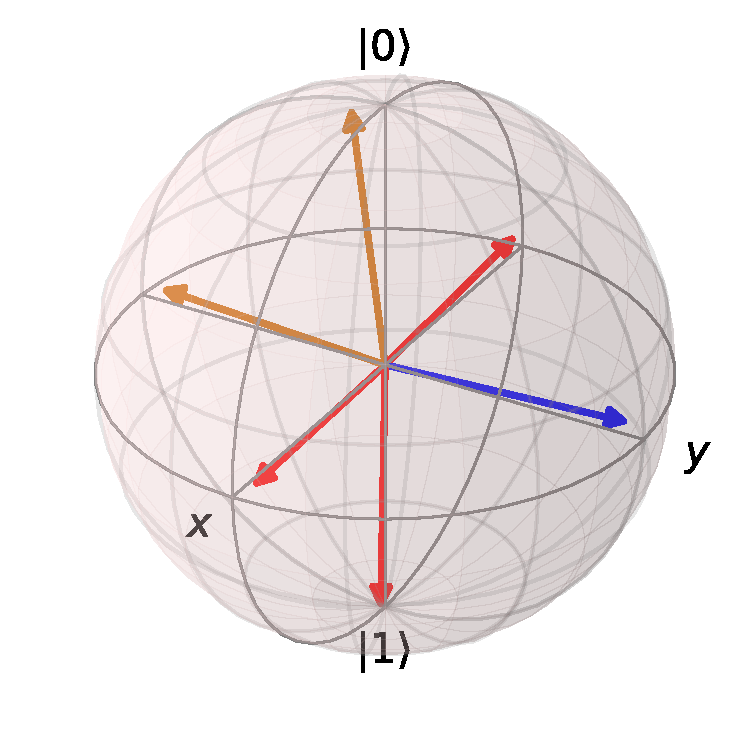
\includegraphics[width=0.25\textwidth]{experimental_study/figures/nv_ga_eval_probes.pdf}
        }
        \qquad
        \subfloat{
            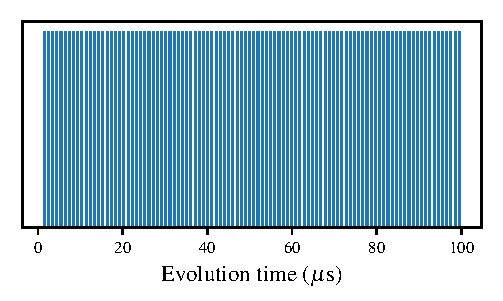
\includegraphics{experimental_study/figures/nv_ga_eval_times.pdf}
        }
    \end{center}
    \caption[Evaluation dataset for nitrogen-vacancy centre genetic algorithm]{
        Evaluation dataset, $\expset_v$, for \acrlong{nvc} \acrlong{ga}. 
        \textbf{Left}, Set of \gls{probe} states the \gls{nvc}  qubit is prepared in for evaluation, 
            i.e. $\Psi_v$ is close to the tomographic basis. 
            Shown are the one-qubit \glspl{probe} on the Bloch sphere, which are combined to form 
            $n$-qubit probes used when evaluating candidate models. 
        \textbf{Right}, Time comb evaluated against, i.e. uniformly distributed times up to $t_{max} = 100 \mu \textrm{s}$ 
            are used for \glspl{experiment} in $\expset_v$. 
        }
    \label{fig:nv_ga_eval_data}
\end{figure}    

\par 

\subsection{Parameter learning}
Our primary goal in this chapter is to validate \gls{qmla}'s performance in a 
    very large \gls{model space}, with over $10^{10}$ valid candidates. 
Our focus, then, is on model \emph{generation}, and not concerned with parameter learning:
    we do \emph{not} train models individually, but rather we assume access to a \emph{perfect} parameter learning subroutine.
That is, for each candidate, $\hi$, considered, we simply assume knowledge of its parameters, $\al_i$. 
This assumption is a major caveat to the results of this chapter: 
    no such perfect training scheme is known, 
    so it remains to examine the detrimental effects of imprecisely finding $\al^{\prime}_i \approx \al_i$. 
Moreover, while it is possible to extract information on the nuclear qubits from measuring only the 
    \gls{nvc} qubit, as in the Hahn echo measurements, 
    it is uncertain whether any technique can simultaneously detect parameters of significantly varying orders of magnitude.
For instance, some terms in \cref{table:nv_gen_alg_term_params} are $\mathcal{O}(\ghz)$, 
    while others are $\mathcal{O}(\khz)$;
    it is likely to prove difficult to discern the $\khz$ parameters well, given that their contribution is equivalent 
    to errors of order $\mathcal{O}(10^{-6})$ in the dominant $\ghz$ terms. 
Therefore we must caution that the results presented here, 
    while demonstrating that \gls{qmla} \emph{can} operate in large model spaces, 
    are not immediately applicable to experimental systems, 
    since there are outstanding challenges in the assessment of individual candidates, 
    which must be overcome before the technique outlined can realistically succeed. 


\subsection{Results}
At the \gls{instance} level, we can see that the gene pool tends towards models of higher quality, 
    captured\footnotemark \ by their \gls{fscore}, \cref{fig:nv_ga_instance}\textbf{(a)}. 
The improvement in modelling is reflected in the branch champions' predictive power at 
    reproducing data generated by the system, \cref{fig:nv_ga_instance}\textbf{(b)}. 
\footnotetext{The use of \gls{fscore} as a figure of merit for candidate models in the \gls{qmla} search is described in \cref{sec:f_score}.}
\begin{figure}
    \begin{center}
        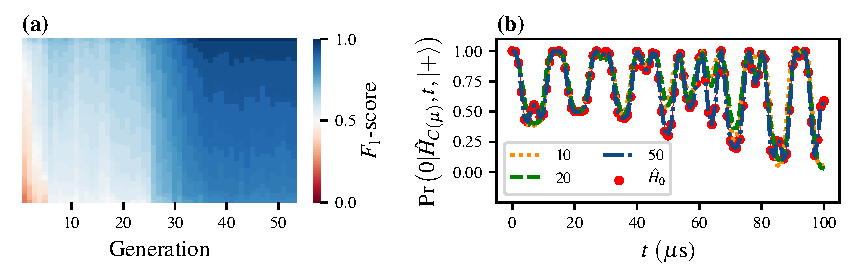
\includegraphics{experimental_study/figures/nv_ga_instance_horiz.pdf}
    \end{center}
    \caption[Instance of genetic algorithm for simulated nitrogen-vacancy centre system with four qubits]{
        \Gls{instance} of the \acrfull{ga} for simulated \acrlong{nvc} system with four qubits.       
        \textbf{a}, Gene pool progression for the \gls{ga}. Each tile represents a candidate model by its \gls{fscore}. 
        Each generation considers $N_m=72$ models; the \gls{ga} runs for $N_g=53$ generations. 
        \textbf{b}, Branch champions' dynamics. 
        Each generation, $\mu$, nominates a branch champion, $\hat{H}_{C(\mu)}$. 
        Here, progressive generations' champions dynamics are shown against those of the target system, $\ho$ (red). 
    }
    \label{fig:nv_ga_instance}
\end{figure}
\par 

Considering the overall \gls{run}, 
    we see that \gls{qmla} is searching in a vast \gls{model space} where randomly sampled models
    have poor \gls{fscore} on average, \cref{fig:nv_ga_run_models}\textbf{(a)}. 
\gls{qmla} efficiently explores the space by quickly moving into a 
    subspace of high \gls{fscore}, nominating $\hp = \ho$ precisely in $85\%$ of instances,
    \cref{fig:nv_ga_run_models}\textbf{(b,c)}.
The number of times each of the terms considered, \cref{eqn:nv_ga_terms}, 
    are present in $\hp$ offers the most important insight from \gls{qmla}, 
    namely the evidence in favour of each term's presence, 
    which can be used to infer the most likely underlying physics. 
Here, $\hat{t} \in \termset_0$ are found in $\geq 94\%$ of instances, 
    while $\hat{t} \notin \termset_0$ are found in $\leq 11\%$, 
    shown in \cref{fig:nv_ga_hinton} and listed in \cref{table:nv_ga_term_counts}.
Such a discrepency, as well as the \glspl{win rate} for the models, 
    allows for the clear declaration of the model $\ho$ as the favoured representation 
    for the quantum system. 
\par 

By simulating a realistic system, we have hereby shown \gls{qmla}'s ability to operate on physically meaningful data
    in large \glspl{model space}. 
The \gls{model search} guided by a \gls{ga} instructs \gls{qmla} to consider only $\sim1000$ models out of the 
    total space of $\sim10^{10}$, 
    clearly showing a drastic speedup in characterising \gls{q} when compared with brute force search.
This demonstration is moderated by the presumptions which enabled us to perform simulations quickly
    and assume perfect outcomes from model training. 
However, taken together with the results of examining experimental data from \cref{chapter:nv}, 
    and the earlier confirmations of \gls{qmla}'s operating principles in \cref{part:theoretical_study}, 
    \gls{qmla} shows promise for characterising genuine small-to-medium quantum systems in the near future. 

\begin{figure}
    \begin{center}
        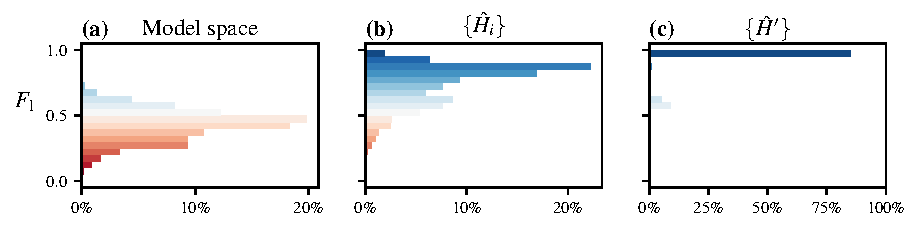
\includegraphics{experimental_study/figures/nv_ga_run_models_by_f.pdf}
    \end{center}
    \caption[Nitrogen-vacancy centre genetic algorithm run]{
        \Acrlong{nvc} \acrlong{ga} \gls{run}.
        \textbf{a}, 
            \gls{fscore} of $10^6$ samples from the \gls{model space} of $2^{33}\approx10^{10}$ candidate models,
            normally distributed around $f=0.44 \pm 0.12$. 
        \textbf{b}, The models explored during the model search of all \glspl{instance} combined, 
            $\{\hat{H}_i\}$, show that \gls{qmla} tends towards stronger models overall, 
            with $f = 0.79 \pm 0.16$ from $\sim 140,000$ chromosomes across the 100 instances, 
            i.e. each \gls{instance} tests $\sim 1400$ distinct models. 
        \textbf{c}, Champion models from each instance, showing \gls{qmla} finds strong models 
            in general, and in particular finds the \gls{true model} ($\ho$, with $f=1$) in $85\%$ of cases.
        }
    \label{fig:nv_ga_run_models}
\end{figure}

\begin{figure}
    \begin{center}
        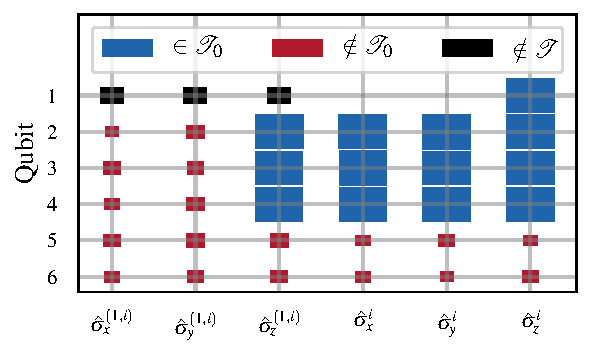
\includegraphics{experimental_study/figures/nv_gen_alg_hinton.pdf}
    \end{center}
    \caption[Hinton diagram of terms found for $4$-qubit nitrogen-vacancy centre model]{
        Hinton diagram of terms found for $4$-qubit \acrlong{nvc} model.
        Terms are either in the target model ($\in \termset_0$, blue) or not ($\notin \termset_0$, red), 
        or else not considered ($\notin \termset$, black). 
        Terms acting solely on the first qubit are the \gls{nvc} spin's rotation terms, $\s_w^1$,
            while each nuclear site also has rotation terms $\s_w^j$.
            Hyperfine terms, $\s_w^{(1,j)}$, couple the \gls{nvc} qubit with the $j^{th}$ nuclear spin. 
            The precise rate at which each term is detected can be read from \cref{table:nv_ga_term_counts}. 
        }
    \label{fig:nv_ga_hinton}
\end{figure}

\begin{table}
    \begin{center}
        \begin{tabular}{lrrrrrr}
\toprule
{} &  $\hat{\sigma}^{(1, i)}_x$ &  $\hat{\sigma}^{(1, i)}_y$ &  $\hat{\sigma}^{(1, i)}_z$ &  $\hat{\sigma}^{i}_x$ &  $\hat{\sigma}^{i}_y$ &  $\hat{\sigma}^{i}_z$ \\
Qubit &                            &                            &                            &                       &                       &                       \\
\midrule
1     &                          - &                          - &                          - &                     0 &                     0 &                   100 \\
2     &                          5 &                         11 &                         97 &                    97 &                    99 &                    97 \\
3     &                         10 &                          9 &                         94 &                    96 &                    94 &                    94 \\
4     &                          7 &                         12 &                         94 &                    94 &                    97 &                    95 \\
5     &                          9 &                         12 &                         11 &                     6 &                     8 &                     5 \\
6     &                          7 &                          9 &                          9 &                     7 &                     5 &                     8 \\
\bottomrule
\end{tabular}

    \end{center}
    \caption[Percentage of instances for which each term is found by QMLA genetic algorithm studying nitrogen-vacancy centre system]{
        Percentage of \glspl{instance} for which each term is found by \gls{qmla} \gls{ga} studying \gls{nvc} system.
    }
    \label{table:nv_ga_term_counts}
\end{table}